%!TEX program = xelatex
\documentclass[a4paper,12pt]{article}
\usepackage{fontspec}\defaultfontfeatures{Ligatures=TeX}
\usepackage[a4paper,vmargin={3cm,3.5cm},hmargin={3cm,3cm}]{geometry}
%-----------------------------------------------------------------------------%
\usepackage{settings}
\setlength{\parindent}{0pt}
%-----------------------------------------------------------------------------%
%%% Title %%%
\title{G6411 Recitation Notes: Weak Instruments}
\author{Jesse Chieh Chen\\\href{mailto:cc5229@columbia.edu}{cc5229@columbia.edu}}
\date{\today}
%-----------------------------------------------------------------------------%

\begin{document}

\maketitle

% The textbook theory of \gls{iv} estimation holds the first stage fixed as $n\to\infty$.
% Any nonzero first-stage coefficient then delivers a consistent and asymptotically normal \gls{tsls} estimator.
% In practice, the excluded instruments often explain little of the variation in the endogenous regressor,
% and the normal approximation can be poor even in very large samples.
% This note explains what goes wrong, how to measure it, and how to do inference that remains valid.
% It follows the notation of the lecture slides and draws on
% \textcite{rothenberg-1984}, \textcite{staiger-stock-1997}, and \textcite{stock-wright-yogo-2002}.

\begin{definition}[\glsentryshort{iv} Model]\label{def-iv-model}
	Let $x_{2i}$ be one endogenous regressor,
	let $x_{1i}\in\reals^{k_1}$ be exogenous regressors
	and let $z_{2i}\in\reals^q$ be excluded instruments:
	\begin{align}
		y_i&=x_{1i}\T\beta_1+x_{2i}\beta_2+e_i,\label{eq-structural}\\
		x_{2i}&=x_{1i}\T\gamma_1+z_{2i}\T\gamma_2+u_i,\label{eq-first-stage}
	\end{align}
	with instruments $z_i=(x_{1i}\T,z_{2i}\T)\T\in\reals^\ell$, $\ell=k_1+q$, and
	$\E(z_ie_i)=0$, $\E(z_iu_i)=0$.
	In matrix form, $y=X_1\beta_1+x_2\beta_2+e$ and $x_2=X_1\gamma_1+Z_2\gamma_2+u$, with $Z=[X_1,Z_2]$.
\end{definition}

\begin{remark}[Partialling Out the Controls]
	Let $M_1=I_n-X_1(X_1\T X_1)\inv X_1\T$.
	By the \gls{fwl} theorem,
	the \gls{tsls} estimator of $\beta_2$ and the other statistics discussed in this note depend on the data only through
	$\tilde y=M_1y$, $\tilde x_2=M_1x_2$, and $\tilde Z_2=M_1Z_2$.
	To keep the algebra short, we therefore drop the controls and the tildes, and write
	\begin{align}\label{eq-simple}
		\begin{aligned}
			y&=x\beta+e \\
			x&=Z\gamma+u
		\end{aligned}
		\quad\text{where}\quad
		Z\in\reals^{n\times q}.
	\end{align}
	Results stated for \eqref{eq-simple} hold for \eqref{eq-structural}-\eqref{eq-first-stage}
	after replacing $Z$ with $\tilde Z_2$ and $n-q$ with $n-\ell$ in degrees of freedom.
\end{remark}

\begin{remark}[One Endogenous Variable]
	\textcite{andrews-stock-sun-2019} survey \gls{iv} specifications in papers published in the \emph{American Economic Review} from 2014 to 2018:
	211 of the 230 specifications (about 92\%) have a single endogenous regressor.
	In general, $x_{2i}$ can be a vector, but we focus on the scalar case throughout.
\end{remark}

\section{A Finite-Sample Primer: The Concentration Parameter}

The \gls{tsls} estimation error is
\begin{align}\label{eq-tsls-error}
	% \widehat\beta_{\mathrm{2SLS}}=\frac{x\T P_Zy}{x\T P_Zx}
	% \quad\text{and}\quad
	\widehat\beta_{\mathrm{2SLS}}-\beta
	=\frac{x\T P_Ze}{x\T P_Zx}
	=\frac{\gamma\T Z\T e+u\T P_Ze}{\gamma\T Z\T Z\gamma+2\gamma\T Z\T u+u\T P_Zu},
\end{align}
where $P_Z=Z(Z\T Z)\inv Z\T$ and $M_Z=I_n-P_Z$.
\textcite{rothenberg-1984} analyzes \eqref{eq-tsls-error} exactly under normality.
The analysis shows that the \emph{concentration parameter}, not sample size, governs the distribution of \gls{tsls}.

\begin{assumption}[Gaussian Errors]\label{ass-gaussian}
	Conditional on $Z$, the pairs $(e_i,u_i)$ are \gls{iid} bivariate normal with mean zero.
	Write $\sigma_e^2=\var(e_i)$, $\sigma_u^2=\var(u_i)$, and $\rho=\operatorname{Corr}(e_i,u_i)$.
\end{assumption}

\begin{definition}
	The \emph{concentration parameter} is
	$\lambda_n={\gamma\T Z\T Z\gamma}/{\sigma_u^2}$.
	% \begin{align}
	% 	\lambda_n=\frac{\gamma\T Z\T Z\gamma}{\sigma_u^2}.
	% \end{align}
\end{definition}

Standardize the terms in \eqref{eq-tsls-error} by defining
\begin{align*}
	\zeta_e=\frac{\gamma\T Z\T e}{\sigma_e\sqrt{\gamma\T Z\T Z\gamma}},\quad
	\zeta_u=\frac{\gamma\T Z\T u}{\sigma_u\sqrt{\gamma\T Z\T Z\gamma}},\quad
	S_{ue}=\frac{u\T P_Ze}{\sigma_u\sigma_e},\quad
	S_{uu}=\frac{u\T P_Zu}{\sigma_u^2}.
\end{align*}
Since $\gamma\T Z\T Z\gamma=\sigma_u^2\lambda_n$, dividing the numerator and denominator of \eqref{eq-tsls-error}
by $\sigma_u^2\lambda_n$ gives
\begin{align}\label{eq-rothenberg}
	\sqrt{\lambda_n}\,(\widehat\beta_{\mathrm{2SLS}}-\beta)
	=\frac{\sigma_e}{\sigma_u}\cdot
	\frac{\zeta_e+S_{ue}/\sqrt{\lambda_n}}{1+2\zeta_u/\sqrt{\lambda_n}+S_{uu}/\lambda_n}.
\end{align}

\begin{proposition}\label{prop-building-blocks}
	Under \autoref{ass-gaussian},
	$(\zeta_e,\zeta_u)$ is bivariate standard normal with correlation $\rho$,
	$S_{uu}\sim\chi^2_q$, and $S_{ue}$ has mean $q\rho$ and variance $q(1+\rho^2)$.
	None of these distributions depends on $n$ or $\gamma$.
\end{proposition}
\begin{proof}
	Let $\eta_e=(Z\T Z)^{-1/2}Z\T e/\sigma_e$ and $\eta_u=(Z\T Z)^{-1/2}Z\T u/\sigma_u$.
	Conditional on $Z$, these are jointly normal $\normaldistribution(0,I_q)$ vectors with $\cov(\eta_e,\eta_u)=\rho I_q$.
	With the unit vector $a=(Z\T Z)^{1/2}\gamma/\|(Z\T Z)^{1/2}\gamma\|$,
	we have $\zeta_e=a\T\eta_e$, $\zeta_u=a\T\eta_u$, $S_{ue}=\eta_u\T\eta_e$, and $S_{uu}=\eta_u\T\eta_u$.
	Each coordinate product $\eta_{u,j}\eta_{e,j}$ has mean $\rho$ and variance
	$\E(\eta_{u,j}^2\eta_{e,j}^2)-\rho^2=(1+2\rho^2)-\rho^2$.
\end{proof}

\begin{remark}[Concentration Parameter as Effective Sample Size]\label{rmk-effective}
	In \eqref{eq-rothenberg},
	the sample size enters \emph{only} through $\lambda_n$.
	As $\lambda_n\to\infty$, the right-hand side tends to $(\sigma_e/\sigma_u)\zeta_e$,
	which is normal, and the usual approximation is accurate.
	When $\lambda_n$ is small, the terms $S_{ue}/\sqrt{\lambda_n}$ and $S_{uu}/\lambda_n$ matter.
	Since $\E(S_{ue})=q\rho$, the numerator is shifted in the direction of $\rho$, which is the direction of the \gls{ols} bias.
	The random denominator also produces skewness and heavy tails.
	Note that $n\to\infty$ does not guarantee $\lambda_n\to\infty$:
	what matters is how much the excluded instruments move $x$, not how many observations there are.
	% The exact distributions are tabulated by \textcite{nelson-startz-1990a,nelson-startz-1990b}.
\end{remark}

\begin{remark}[Concentration Parameter as First-Stage $F$-Statistic]\label{rmk-first-stage-f}
	The first-stage $F$-statistic is
	\begin{align*}
		F=\frac{x\T P_Zx/q}{x\T M_Zx/(n-q)}.
	\end{align*}
	Under \autoref{ass-gaussian}, $x\T P_Zx/\sigma_u^2\sim\chi^2_q(\lambda_n)$, a noncentral chi-squared distribution,
	and it is independent of $x\T M_Zx/\sigma_u^2\sim\chi^2_{n-q}$.
	Hence $F\given Z\sim F_{q,n-q}(\lambda_n)$ exactly, a noncentral $F$ distribution, and
	\begin{align*}
		\E \left(\frac{x\T P_Z x/q}{\sigma_u^2}\right)
		= 1 + \frac{\lambda_n}{q}.
	\end{align*}
	Since the denominator of $F$ has probability limit $\sigma_u^2$, $\E(F)-1\approx\lambda_n/q$ for large $n$:
	the concentration parameter per instrument.
	The statistic $F$ itself is noisy, so a single $F$ only indicates the size of $\lambda_n/q$.
	A small first-stage $F$ signals a small $\lambda_n$, and therefore that \eqref{eq-rothenberg} is far from normal.
\end{remark}

\begin{remark}[Vector Form]\label{rmk-vector-form}
	We can rewrite \eqref{eq-rothenberg} in vector form, which is useful for general $q$.
	With $\eta_e$ and $\eta_u$ as in the proof of \autoref{prop-building-blocks},
	writing $\nu_n=(Z\T Z)^{1/2}\gamma/\sigma_u$, so that $\nu_n\T\nu_n=\lambda_n$,
	the identity $(Z\T Z)^{-1/2}Z\T x=\sigma_u(\nu_n+\eta_u)$ turns \eqref{eq-tsls-error} into
	\begin{align}\label{eq-rothenberg-vector}
		\widehat\beta_{\mathrm{2SLS}}-\beta
		=\frac{\sigma_e}{\sigma_u}\cdot
		\frac{(\nu_n+\eta_u)\T\eta_e}{(\nu_n+\eta_u)\T(\nu_n+\eta_u)}.
	\end{align}
	This is an exact finite-sample representation, and it is equivalent to \eqref{eq-rothenberg}.
	The pair $(\eta_e,\eta_u)$ has a fixed distribution, so $\lambda_n$ (through $\nu_n$) is the only thing that changes with the design.
\end{remark}

\section{Weak-Instrument Asymptotics}

The finite-sample theory of \textcite{rothenberg-1984} needs normality.
\textcite{staiger-stock-1997} propose an asymptotic framework that reproduces the same features without these assumptions.
The idea is to let the first stage shrink with $n$, so that $\lambda_n$ stays bounded instead of exploding.

\begin{assumption}[Local-to-Zero First Stage]\label{ass-weak}
	The first-stage coefficient is $\gamma=\gamma_n=c/\sqrt n$ for a fixed $c\in\reals^q$.
	The observations are \gls{iid}, $Z\T Z/n\pto Q>0$,
	$\E\bigl((e_i,u_i)\T(e_i,u_i)\given z_i\bigr)=\Sigma$ with variances $\sigma_e^2,\sigma_u^2$ and correlation $\rho$,
	and
	\begin{align*}
		\frac{1}{\sqrt n}\begin{pmatrix}Z\T e\\Z\T u\end{pmatrix}
		\dto
		\begin{pmatrix}\xi_e\\\xi_u\end{pmatrix}
		\sim\normaldistribution(0,\Sigma\otimes Q)
		\quad\text{where}\quad
		\Sigma\otimes Q=
		\begin{pmatrix}
			\sigma_e^2 Q & \rho\sigma_e\sigma_u Q\\
			\rho\sigma_e\sigma_u Q & \sigma_u^2 Q
		\end{pmatrix}.
	\end{align*}
\end{assumption}

\begin{remark}[What Does $\gamma_n=c/\sqrt{n}$ Mean?]
	The drift $\gamma_n=c/\sqrt n$ is not a claim that first-stage coefficients shrink in reality.
	Asymptotic theory is a device for approximating finite-sample distributions, and it is useful only if the approximation is good.
	Under a fixed first stage, $\lambda_n$ diverges;
	the drift instead keeps $\lambda_n$ of the same order as in the sample at hand, so the limit inherits the finite-sample behavior we care about.
	\autoref{thm-staiger-stock} below shows that it reproduces the representation of \textcite{rothenberg-1984}.
\end{remark}

\begin{lemma}
	$\lambda_n\pto\lambda$ where $\lambda=c\T Qc/\sigma_u^2<\infty$.
\end{lemma}
\begin{proof}
	Since $Z\T Z/n\pto Q$, $\lambda_n=c\T(Z\T Z/n)c/\sigma_u^2\pto c\T Qc/\sigma_u^2$.
\end{proof}

% So the concentration parameter is held fixed, while it would diverge with a fixed first stage.
% The drift $c/\sqrt n$ is not a claim that coefficients shrink in reality.
% It is a device that keeps $\lambda_n$ of the same order as in the sample at hand,
% so the limit inherits the finite-sample behavior we care about.

% \subsection{The Scalar Case: $q=1$}

\begin{proposition}[Simplified Case with $q=1$]\label{prop-scalar}
	Consider a simplified case with $q=1$, $\E(z_i^2)=1$, and $\sigma_e=\sigma_u=1$,
	so that $c$ is a scalar, $x_i=z_ic/\sqrt n+u_i$, and $\lambda=c^2$.
	Under \autoref{ass-weak} with $q=1$,
	\begin{align}
		\widehat\beta_{\mathrm{OLS}}\pto\beta+\rho,
		\qquad
		\widehat\beta_{\mathrm{IV}}-\beta\dto\frac{\xi_e}{c+\xi_u},
		\qquad
		\begin{pmatrix}\xi_e\\\xi_u\end{pmatrix}
		\sim\normaldistribution\left(0,\begin{pmatrix}1&\rho\\\rho&1\end{pmatrix}\right).
	\end{align}
\end{proposition}
\begin{proof}
	For \gls{ols}, the signal vanishes from both sample averages:
	$n\inv\sum_ix_ie_i=c\,n^{-3/2}\sum_iz_ie_i+n\inv\sum_iu_ie_i\pto\rho$,
	and similarly $n\inv\sum_ix_i^2\pto1$.
	For \gls{iv}, multiply the numerator and denominator by $n^{-1/2}$:
	\begin{align*}
		\widehat\beta_{\mathrm{IV}}-\beta
		=\frac{n^{-1/2}\sum_iz_ie_i}{c\,n\inv\sum_iz_i^2+n^{-1/2}\sum_iz_iu_i}
		\dto\frac{\xi_e}{c+\xi_u}
	\end{align*}
	by the continuous mapping theorem.
\end{proof}

\begin{remark}[Interpretation]\label{rmk-interpretation}
	\autoref{prop-scalar} has several implications:
	\begin{enumerate}
		\item \gls{iv} is \emph{inconsistent}: it converges in distribution to a random variable, not to $\beta$.
		\item The limit is nonnormal. When $c+\xi_u$ is near zero, the estimate can be extreme.
		\item At $c=0$ and $\rho=0$, the limit $\xi_e/\xi_u$ is standard Cauchy and has no mean.
		\item When $c$ is small (well below one, so $\lambda\ll1$), the limit is centered near $\rho$, the \gls{ols} bias.
		Decompose $\xi_e=\rho\xi_u+\sqrt{1-\rho^2}\,\varepsilon$, where $\varepsilon\sim\normaldistribution(0,1)$ is independent of $\xi_u$. Then
		\begin{align*}
			\frac{\xi_e}{c+\xi_u}
			=\rho\cdot\frac{\xi_u}{c+\xi_u}
			+\sqrt{1-\rho^2}\cdot\frac{\varepsilon}{c+\xi_u}.
		\end{align*}
		As $c\to0$, the first term tends to $\rho$,
		and the second term is symmetric around zero given $\xi_u$.
		At $c=0$, the limit is $\rho$ plus a scaled Cauchy variable, with median $\rho$:
		\gls{iv} is centered at the \gls{ols} probability limit $\beta+\rho$.
		\item As $c\to\infty$, $c\cdot\xi_e/(c+\xi_u)\to\xi_e\sim\normaldistribution(0,1)$, recovering the textbook result.
	\end{enumerate}
\end{remark}

For general $q$, define $\eta_e=Q^{-1/2}\xi_e/\sigma_e$, $\eta_u=Q^{-1/2}\xi_u/\sigma_u$, and $\nu=Q^{1/2}c/\sigma_u$.
Then, the weak \gls{iv} asymptotic limit mimics the finite-sample representation \eqref{eq-rothenberg-vector}:

\begin{theorem}[\cite{staiger-stock-1997}]\label{thm-staiger-stock}
	Under \autoref{ass-weak},
	\begin{align}\label{eq-staiger-stock}
		\widehat\beta_{\mathrm{2SLS}}-\beta
		\dto\frac{\sigma_e}{\sigma_u}\cdot
		\frac{(\nu+\eta_u)\T\eta_e}{(\nu+\eta_u)\T(\nu+\eta_u)},
	\end{align}
	where $\eta_e,\eta_u\sim\normaldistribution(0,I_q)$ with $\cov(\eta_e,\eta_u)=\rho I_q$, and $\nu\T\nu=\lambda$.
\end{theorem}
\begin{proof}
	Write
	\begin{align*}
		\widehat\beta_{\mathrm{2SLS}}-\beta
		=\frac{(n^{-1/2}x\T Z)(Z\T Z/n)\inv(n^{-1/2}Z\T e)}{(n^{-1/2}x\T Z)(Z\T Z/n)\inv(n^{-1/2}Z\T x)}.
	\end{align*}
	Since $n^{-1/2}Z\T x=(Z\T Z/n)c+n^{-1/2}Z\T u\dto Qc+\xi_u=\sigma_uQ^{1/2}(\nu+\eta_u)$
	and $n^{-1/2}Z\T e\dto\sigma_eQ^{1/2}\eta_e$, the result follows from the continuous mapping theorem.
\end{proof}

\begin{remark}
	Compare \eqref{eq-staiger-stock} with the exact finite-sample representation \eqref{eq-rothenberg-vector}.
	They have the \emph{same form}, with $\nu_n$ replaced by its limit $\nu$.
	This is the sense in which weak-instrument asymptotics mimic the finite-sample distribution of \textcite{rothenberg-1984}:
	the limit keeps the concentration parameter fixed at $\lambda=\nu\T\nu$, and nothing else about the design matters.
	The difference is that \eqref{eq-staiger-stock} needs neither normal errors nor fixed instruments,
	although it still uses the conditional homoskedasticity in \autoref{ass-weak}.
\end{remark}

% \begin{remark}[Relative Bias]\label{rmk-relative-bias}
% 	Under \autoref{ass-weak}, $\widehat\beta_{\mathrm{OLS}}-\beta\pto\rho\sigma_e/\sigma_u$.
% 	Averaging the limit \eqref{eq-staiger-stock} over the part of $\eta_e$ that is independent of $\eta_u$,
% 	the bias of \gls{tsls} relative to \gls{ols} is
% 	\begin{align*}
% 		\E\left[\frac{(\nu+\eta_u)\T\eta_u}{(\nu+\eta_u)\T(\nu+\eta_u)}\right],
% 	\end{align*}
% 	whenever this expectation exists.
% 	It depends only on $\lambda/q$ and $q$.
% 	At $\lambda=0$ (irrelevant instruments), it equals one: \gls{tsls} is centered at the \gls{ols} probability limit.
% 	For $\lambda>0$, \gls{tsls} is centered between $\beta$ and the \gls{ols} limit, approaching $\beta$ as $\lambda/q$ grows.
% \end{remark}

\begin{remark}[Why $\lambda$ Cannot Be Estimated Away]
	Under \autoref{ass-weak}, $qF\dto(\nu+\eta_u)\T(\nu+\eta_u)\sim\chi^2_q(\lambda)$.
	So $F$ is informative about $\lambda$ but does not converge to it.
	No consistent estimator of $\lambda$ exists in this framework,
	so one cannot simply plug in an estimate of $\lambda$ and use \eqref{eq-staiger-stock} to construct critical values.
	This is also why it is not very meaningful to ask how large $c$ is in a given application:
	$c$ is a device of the asymptotic sequence, not a feature of the data.
\end{remark}

\subsection{The \texorpdfstring{$t$}{t}-Statistic under Weak-\glsentryshort{iv} Asymptotics}

Recall that, under homoskedasticity, the $t$-statistic for \gls{iv} (with $q=1$) is
\begin{align*}
	T_n=\frac{\widehat\beta_{\mathrm{IV}}-\beta}{\operatorname{se}(\widehat\beta_{\mathrm{IV}})}
	\quad\text{where}\quad
	\widehat\var(\widehat\beta_{\mathrm{IV}})
	= \widehat\sigma_e^2 (x\T P_Zx)\inv,
	\quad
	\widehat\sigma_e^2 = \frac1n\sum_i(y_i-x_i\widehat\beta_{\mathrm{IV}})^2.
\end{align*}

\begin{proposition}[Weak-\glsentryshort{iv} Limit of the $t$-Statistic]
	Under the assumptions of \autoref{prop-scalar},
	\begin{align}
		T_n = \frac{\widehat\beta_{\mathrm{IV}}-\beta}{\operatorname{se}(\widehat\beta_{\mathrm{IV}})}
		\dto\frac{\operatorname{sign}(c+\xi_u)\,\xi_e}{\sqrt{1-2\rho\Delta+\Delta^2}},
	\end{align}
	where $\Delta=\xi_e/(c+\xi_u)$ denotes the limit of $\widehat\beta_{\mathrm{IV}}-\beta$.
\end{proposition}
\begin{proof}
	Since $y_i-x_i\widehat\beta_{\mathrm{IV}}=e_i-x_i(\widehat\beta_{\mathrm{IV}}-\beta)$,
	\begin{align*}
		\widehat\sigma_e^2
		=\frac1n\sum_ie_i^2-2(\widehat\beta_{\mathrm{IV}}-\beta)\frac1n\sum_ix_ie_i+(\widehat\beta_{\mathrm{IV}}-\beta)^2\frac1n\sum_ix_i^2,
	\end{align*}
	and the three sample averages converge to $1$, $\rho$, and $1$.
	Next,
	\begin{align*}
		x\T P_Zx&=\frac{(n^{-1/2}\sum_iz_ix_i)^2}{n\inv\sum_iz_i^2}\dto(c+\xi_u)^2,\\
		T_n&=\frac{(\widehat\beta_{\mathrm{IV}}-\beta)\sqrt{x\T P_Zx}}{\widehat\sigma_e}
		\dto\frac{\Delta\,|c+\xi_u|}{\sqrt{1-2\rho\Delta+\Delta^2}},
	\end{align*}
	jointly, and $\Delta\,|c+\xi_u|=\operatorname{sign}(c+\xi_u)\,\xi_e$.
\end{proof}

\begin{remark}[Over-Rejection of the $t$-Test]
	The residual variance does not converge to $\sigma_e^2=1$:
	because $\widehat\beta_{\mathrm{IV}}$ is inconsistent, the residuals contain $-x_i(\widehat\beta_{\mathrm{IV}}-\beta)$,
	which does not vanish.
	The $t$-statistic's limit is nonnormal and depends on $c$ and $\rho$.
	When $c$ is small, $\Delta$ is centered near $\rho$ (\autoref{rmk-interpretation}),
	and at $\Delta=\rho$ the limit of $\widehat\sigma_e^2$ is $1-2\rho^2+\rho^2=1-\rho^2$.
	With $\rho=0.9$, for example, $\widehat\sigma_e^2$ is around $0.19$ instead of $1$.
	The standard error is then far too small, which makes the $t$-test over-reject.
	As $c\to\infty$, $\Delta\to0$ and $T_n\dto\xi_e\sim\normaldistribution(0,1)$.
\end{remark}

\subsection{Where This Leaves Us}

Weak-instrument asymptotics do not produce a new estimator or a usable test.
They establish a \emph{regime} in which the failures of the textbook approximation are visible,
so that diagnostics and inference procedures can be evaluated within it.

\begin{remark}[How Do We Proceed?]
	There are two general types of response to weak instruments \parencite{stock-wright-yogo-2002}:
	\begin{enumerate}
		\item Pretest the first stage, and use conventional inference only if the instruments are strong enough (\autoref{sec-stock-yogo}).
		\item Use tests whose size is correct \emph{regardless} of instrument strength. This is known as \emph{robust} testing (\autoref{sec-ar}).
	\end{enumerate}
\end{remark}

\section{Testing for Weak Instruments: \texorpdfstring{\textcite{stock-yogo-2005}}{Stock and Yogo (2005)}}\label{sec-stock-yogo}

From here on we return to the full model \eqref{eq-structural}-\eqref{eq-first-stage} with controls,
so $Z=[X_1,Z_2]$, the coefficients of interest are $\beta_2$ and $\gamma_2$,
and the concentration parameter is computed with $\tilde Z_2$ in place of $Z$.

\begin{table}[ht]
	\centering
	\begin{tabular}{ccccc}
		\toprule
		$q$ & $\bar r=10\%$ & $\bar r=15\%$ & $\bar r=20\%$ & $\bar r=25\%$\\
		\midrule
		1 & 16.38 & 8.96 & 6.66 & 5.53\\
		2 & 19.93 & 11.59 & 8.75 & 7.25\\
		4 & 24.58 & 13.96 & 10.26 & 8.31\\
		10 & 38.54 & 20.88 & 14.78 & 11.65\\
		\bottomrule
	\end{tabular}
	\caption{Critical values for the 5\% weak-instrument test based on \gls{tsls} size, with one endogenous regressor.
	Weakness is rejected if the first-stage $F$ exceeds the critical value;
	$\bar r$ is the tolerated maximal size of a nominal 5\% Wald test of $H_0:\beta_2=b_0$.
	Source: \textcite[Table 2]{stock-yogo-2005}.}
	\label{tab-stock-yogo}
\end{table}

The conventional first-stage $F$ test of $H_0:\gamma_2=0$ is a test of \emph{relevance}.
Rejecting it only says the instruments are not completely irrelevant.
\textcite{stock-yogo-2005} instead test whether the instruments are \emph{weak}, defined by a tolerance for a specific failure.

\begin{definition}[Weak Instruments, Size-Based]
	Fix a nominal 5\% Wald test of $H_0:\beta_2=b_0$ and a tolerance $\bar r$ (for example, $10\%$ or $15\%$).
	The instruments are \emph{weak} if the maximal actual rejection rate of this test under $H_0$,
	maximized over the degree of endogeneity $\rho$ under weak-instrument asymptotics, exceeds $\bar r$.
\end{definition}

\begin{remark}[From a Size Tolerance to a Critical Value]
	Take $\bar r=10\%$.
	The instruments are weak if a nominal 5\% \gls{tsls} Wald test could reject a \emph{true} null more than 10\% of the time.
	Under weak-instrument asymptotics, this worst-case rejection rate depends only on $q$ and $\lambda/q$,
	and it falls as $\lambda/q$ grows.
	So ``weak'' means $\lambda/q$ lies below a threshold that depends on $\bar r$ and $q$:
	a stricter tolerance (smaller $\bar r$) requires a larger $\lambda/q$.
	Stock and Yogo then test
	\begin{align*}
		H_0:\text{instruments are weak}
		\qquad\text{against}\qquad
		H_1:\text{instruments are not weak}
	\end{align*}
	using the first-stage $F$, whose distribution depends on $\lambda$ (\autoref{rmk-first-stage-f}).
	The critical value is set so that, at the boundary value of $\lambda/q$, the probability that $F$ exceeds it is 5\%.
	A first-stage $F$ above the critical value therefore rejects weakness at the 5\% level.
	The critical value depends on $\bar r$, the estimator, $q$, and the number of endogenous regressors.
\end{remark}

\begin{example}[Reading the Table]
	Suppose $q=4$ and the first-stage $F$ is $15$.
	At tolerance $\bar r=10\%$, the critical value is $24.58>15$, so we cannot reject that the instruments are weak:
	a nominal 5\% \gls{tsls} Wald test might reject more than 10\% of the time.
	At $\bar r=15\%$, the critical value is $13.96<15$, so we reject weakness at that looser tolerance.
\end{example}

\begin{remark}[Caveats]
	A few cautions apply when using these tables.
	\begin{enumerate}
		\item The critical values grow with $q$ for \gls{tsls}, since its size distortion grows with the number of instruments.
		For \gls{liml}, they fall with $q$ over most of the tabulated range (at $\bar r=10\%$, down to $q\approx19$),
		consistent with \autoref{sec-liml}.
		With $q=1$, \gls{iv}, \gls{tsls}, and \gls{liml} coincide, and so do the critical values.
		\item With one or two instruments, the popular rule of thumb $F>10$ \parencite{staiger-stock-1997}
		corresponds roughly to the $\bar r=15\%$ benchmark.
		With more instruments, the critical values are much larger, and $F>10$ gives little assurance that the size distortion is controlled \parencite{stock-yogo-2005}.
		\item The tables assume homoskedastic, serially uncorrelated errors.
		They do not automatically apply to a heteroskedasticity-robust $F$ statistic.
		\item Pretesting and then using conventional inference only when $F$ is large is itself a two-step procedure,
		whose overall size is not controlled exactly.
	\end{enumerate}
\end{remark}

\section{Fully Robust Inference}\label{sec-ar}

If $\gamma_2=0$, $\beta_2$ is not identified.
Consequently, no estimator has a $t$-statistic that is approximately normal regardless of instrument strength.
There are, however, robust \emph{tests} of $H_0:\beta_2=b_0$,
whose null distribution does not depend on instrument strength.

\subsection{The Anderson-Rubin Test}

The idea of \textcite{anderson-rubin-1949} is to impose the null before looking at the instruments.
Under $H_0:\beta_2=b_0$,
\begin{align}
	r(b_0)=y-x_2b_0=X_1\beta_1+e,
\end{align}
so the excluded instruments should have zero coefficients in the regression
\begin{align}\label{eq-ar-regression}
	r(b_0)=X_1a+Z_2\delta+\text{error},
\end{align}
that is, $\delta=0$ under $H_0$.
In other words, we simply test for correlation between the excluded instruments and the structural error implied by the null.
No first-stage coefficient appears.

\begin{definition}[\glsentryshort{ar} Statistic]
	With $P_1=X_1(X_1\T X_1)\inv X_1\T$,
	\begin{align}
		\mathrm{AR}(b_0)=\frac{r(b_0)\T(P_Z-P_1)r(b_0)/q}{r(b_0)\T M_Zr(b_0)/(n-\ell)}.
	\end{align}
\end{definition}

\begin{theorem}[Exact Null Distribution]\label{thm-ar-exact}
	If $e\given Z\sim\normaldistribution(0,\sigma_e^2I_n)$, then under $H_0:\beta_2=b_0$,
	$\mathrm{AR}(b_0)\sim F_{q,n-\ell}$, whatever the value of $\gamma_2$.
\end{theorem}
\begin{proof}
	Under $H_0$, $r(b_0)=X_1\beta_1+e$, and both $P_Z-P_1$ and $M_Z$ annihilate $X_1$, so
	$r\T(P_Z-P_1)r=e\T(P_Z-P_1)e$ and $r\T M_Zr=e\T M_Ze$.
	The two matrices are symmetric idempotent with ranks $q$ and $n-\ell$, and $(P_Z-P_1)M_Z=0$.
	So, divided by $\sigma_e^2$, the two quadratic forms are independent $\chi^2_q$ and $\chi^2_{n-\ell}$ variables.
	No first-stage parameter enters.
\end{proof}

\begin{remark}[The \glsentryshort{ar} Statistic Is an $F$-Statistic]
	The \gls{ar} statistic is simply the $F$-statistic for testing $\delta=0$ in \eqref{eq-ar-regression}.
	Without normality, $q\,\mathrm{AR}(b_0)\dto\chi^2_q$ under $H_0$, under both strong and weak-instrument asymptotics.
	With heteroskedasticity, serial correlation, or clustering, replace the $F$-statistic with a robust Wald statistic for $\delta=0$ in \eqref{eq-ar-regression}.
\end{remark}

\begin{remark}[The \glsentryshort{ar} Statistic and the Reduced Form]\label{rmk-ar-reduced-form}
	Substituting the first stage \eqref{eq-first-stage} into the structural equation \eqref{eq-structural} gives the reduced form for $y$:
	\begin{align*}
		y=X_1\pi_1+Z_2\pi_2+(e+u\beta_2),
		\qquad
		\pi_1=\beta_1+\gamma_1\beta_2,
		\quad
		\pi_2=\gamma_2\beta_2.
	\end{align*}
	Regress $y$ and $x_2$ on $(X_1,Z_2)$, and let $\widehat\pi_2$ and $\widehat\gamma_2$ be the coefficients on $Z_2$.
	By the \gls{fwl} theorem, with $\tilde Z_2=M_1Z_2$,
	\begin{align*}
		\widehat\pi_2=(\tilde Z_2\T\tilde Z_2)\inv\tilde Z_2\T y,
		\qquad
		\widehat\gamma_2=(\tilde Z_2\T\tilde Z_2)\inv\tilde Z_2\T x_2.
	\end{align*}
	The coefficient on $Z_2$ in \eqref{eq-ar-regression} is therefore
	\begin{align*}
		\widehat\delta(b_0)
		=(\tilde Z_2\T\tilde Z_2)\inv\tilde Z_2\T(y-x_2b_0)
		=\widehat\pi_2-\widehat\gamma_2b_0.
	\end{align*}
	Its population counterpart is $\pi_2-\gamma_2b_0=\gamma_2(\beta_2-b_0)$, which is zero under $H_0$ for \emph{every} $\gamma_2$, including $\gamma_2=0$.
	Since $P_Z-P_1=\tilde Z_2(\tilde Z_2\T\tilde Z_2)\inv\tilde Z_2\T$,
	the numerator of the \gls{ar} statistic is
	\begin{align*}
		r(b_0)\T(P_Z-P_1)r(b_0)
		=\widehat\delta(b_0)\T(\tilde Z_2\T\tilde Z_2)\,\widehat\delta(b_0).
	\end{align*}
	So the \gls{ar} test checks whether $\widehat\pi_2-\widehat\gamma_2b_0$ is close to zero, which is linear in $b_0$.
	Compare this with \gls{iv} when $q=1$: it solves $\widehat\pi_2=\widehat\gamma_2b$ for $b$, giving $\widehat\beta_{\mathrm{IV}}=\widehat\pi_2/\widehat\gamma_2$,
	and dividing by $\widehat\gamma_2$ is exactly what goes wrong when $\gamma_2$ is close to zero.
\end{remark}

\begin{remark}[Shape of \glsentryshort{ar} Confidence Sets]
	Inverting the test gives the confidence set $C_{\mathrm{AR}}=\{b:\mathrm{AR}(b)\le F_{q,n-\ell;1-\alpha}\}$,
	which has exact coverage $1-\alpha$ under the conditions of \autoref{thm-ar-exact}, for every $\gamma_2$.
	The numerator and denominator of $\mathrm{AR}(b)$ are both quadratic in $b$,
	so $\mathrm{AR}(b)\le F_{q,n-\ell;1-\alpha}$ is a quadratic inequality in $b$.
	Its solution set can fall into three categories:
	\begin{enumerate}
		\item A bounded interval, typical when the instruments are strong;
		\item The union of two unbounded rays, or the whole real line, when the instruments are weak;
		\item Empty, in over-identified models, when no value of $b$ fits the $q$ moment conditions well enough.
	\end{enumerate}
	Unbounded sets are not a defect.
	\textcite{dufour-1997} shows that any confidence set with correct coverage for every $\gamma_2$ must be unbounded with positive probability,
	since $\beta_2$ is not identified at $\gamma_2=0$.
	A conventional Wald interval $\widehat\beta_{\mathrm{2SLS}}\pm1.96\operatorname{se}(\widehat\beta_{\mathrm{2SLS}})$ is always bounded, which is one way to see why it cannot have correct coverage.
\end{remark}

\begin{remark}[Power]
	When $q=1$, the \gls{ar} test is the uniformly most powerful unbiased test \parencite{moreira-2009}.
	When $q>1$, it tests more than we want.
	Since $\pi_2=\gamma_2\beta_2$ (\autoref{rmk-ar-reduced-form}), $\delta=\gamma_2(\beta_2-b_0)$:
	only the scale of $\delta$ along $\gamma_2$ is informative about $\beta_2$,
	while the other $q-1$ directions are over-identifying restrictions that hold for any $b_0$.
	Yet the $\chi^2_q$ critical value must absorb the noise in all $q$ directions,
	so, holding $\lambda_n$ fixed, power falls as $q$ grows.
\end{remark}

\subsection{Beyond \glsentryshort{ar}: Over-Identified Models}
The \gls{clr} test of \textcite{moreira-2003} is another route to weak-instrument-robust inference,
with better power than \gls{ar} in over-identified models.
\begin{itemize}
	\item The null distribution of its statistic depends on the first-stage strength.
	But in the canonical Gaussian model, its distribution \emph{conditional on} an observed statistic that carries the first-stage information no longer depends on it.
	\item So its critical values depend on that observed statistic, rather than being a fixed $\chi^2$ cutoff.
	\item The classical construction assumes a homoskedastic reduced-form covariance.
	With heteroskedastic or clustered errors, it requires a robust extension;
	\textcite{andrews-stock-sun-2019} survey current practice.
\end{itemize}
With homoskedastic errors and one endogenous regressor, \gls{clr} is close to optimal.
The over-identified case with heteroskedastic, serially correlated, or clustered errors,
and the case of multiple endogenous regressors, remain active areas of research \parencite{andrews-stock-sun-2019}.

\section{Is \glsentryshort{liml} Robust to Weak Instruments?}\label{sec-liml}

No, but it behaves very differently from \gls{tsls}.
In the notation of \eqref{eq-simple}, both are $k$-class estimators,
\begin{align*}
	\widehat\beta(\kappa)=\bigl(x\T(I_n-\kappa M_Z)x\bigr)\inv x\T(I_n-\kappa M_Z)y,
\end{align*}
with $\kappa=1$ for \gls{tsls}.
\gls{liml} uses $\kappa=\widehat\kappa$, the smallest eigenvalue of $(W\T M_ZW)\inv W\T W$ with $W=[y,x]$,
which is the minimized \gls{liml} criterion and satisfies $\widehat\kappa\ge1$.
\begin{itemize}
	\item With $q=1$, $\widehat\kappa=1$ and \gls{liml} equals \gls{iv}.
		It shares every weak-instrument problem above.
	\item With $q>1$, \gls{liml} is much less biased than \gls{tsls}: it is approximately median-unbiased unless $\lambda$ is very small.
		When the instruments are irrelevant ($\lambda=0$), it is centered at the \gls{ols} probability limit, just like \gls{tsls}.
		The cost is heavy tails. \gls{liml} has no finite moments, so it occasionally produces extreme estimates.
	\item The weak-instrument limit of \gls{liml} still depends on $\lambda$, so conventional \gls{liml} inference is not robust.
		It is, however, much less distorted than \gls{tsls}, which is why its Stock-Yogo critical values are so much smaller:
		with $q=4$ and $\bar r=10\%$, the critical value is $5.44$ for \gls{liml} against $24.58$ for \gls{tsls} \parencite[Tables 2 and 4]{stock-yogo-2005}.
\end{itemize}

\begin{figure}[t]
	\centering
	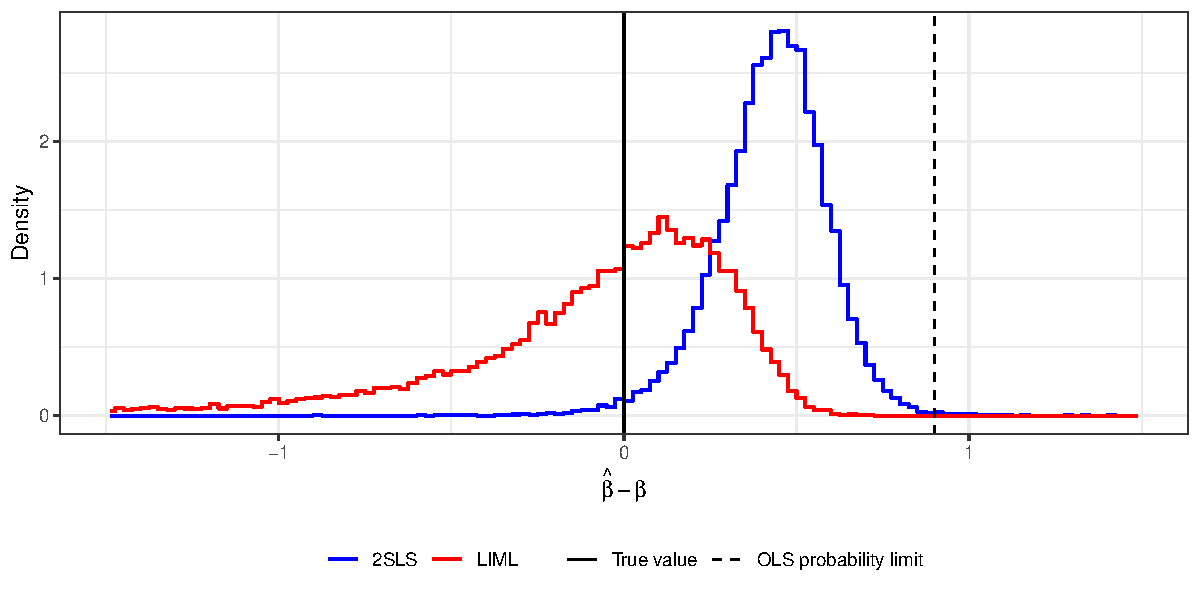
\includegraphics[width=0.8\linewidth]{code/liml-vs-2sls.pdf}
	\caption{Simulated distributions of $\widehat\beta-\beta$ for \gls{tsls} and \gls{liml}
	with $q=10$ instruments and concentration parameter $\lambda=10$
	($n=500$, $\rho=0.9$, $\sigma_e=\sigma_u=1$, $20{,}000$ replications).
	The solid line marks the true value; the dashed line is the \gls{ols} probability limit, $\rho\sigma_e/\sigma_u=\rho$, under weak-instrument asymptotics.}
	\label{fig-liml}
\end{figure}

\begin{remark}[Simulation]
	\autoref{fig-liml} illustrates this with $q=10$ instruments and $\lambda=10$, so $\lambda/q=1$ and the mean first-stage $F$ is about $2$.
	\gls{tsls} is concentrated but centered far from $\beta$: its median bias is $0.44$, about half of the \gls{ols} bias $\rho=0.9$.
	\gls{liml} is centered near $\beta$, with a median bias of $0.005$, but has a long left tail.
	In the same simulation, a nominal 5\% \gls{tsls} $t$-test rejects the true null 74\% of the time,
	a \gls{liml} $t$-test 10\% of the time, and the \gls{ar} test 5.2\% of the time.
	Only the \gls{ar} test has correct size.
\end{remark}

\vfill
\section*{Acronyms}
\printglossaries

\printbibliography[heading=bibintoc,title={References}]

\end{document}
